\section{gufi\_query}

\subsection{Outline}

gufi\_query is used in order to query information from the generated databases that include all of the information about the indexed root directory and its sub-directories while also taking into account permissions 
\subsection{Flags}

\begin{table} [h]
\centering
\begin{tabular}{l|p{6cm}}
Flag & Functionality \\\hline
-h & help\\
\hline
-H & show assigned input values (debugging)\\
\hline
-E \textless SQL ent\textgreater & SQL for entries table \\
\hline
-S \textless SQL sum\textgreater (will be read first) & SQL for summary table\\
\hline
-T \textless SQL tsum\textgreater & SQL for tree-summary table\\
\hline
-a & AND/OR (SQL query combination)\\
\hline
-n \textless threads\textgreater & number of threads\\
\hline
-j & print the information in terse form\\
\hline
-o \textless out\_fname\textgreater & output file (one-per thread, with thread-id suffix) implies -e 1\\
\hline
-d \textless delim\textgreater & one char delimiter \\
\hline
-O \textless out\_DB\textgreater & output DB, implies -e 1 \\
\hline
-I \textless SQL\_init\textgreater & SQL init \\
\hline
-F \textless SQL\_fin\textgreater & SQL cleanup \\
\hline
-y \textless min-level\textgreater & minimum level to descend to \\
\hline
-z \textless max-level\textgreater & maximum level to descend to\\
\hline
-J \textless SQL\_interm\textgreater & SQL for intermediate results (no default: recommend using "SELECT * FROM entries") \\
\hline
-K \textless create aggregate\textgreater & SQL to create the final aggregation table (if not specified, -I will be used)\\
\hline
-G \textless SQL\_aggregate\textgreater & SQL for aggregated results (no default: recommend using "SELECT * FROM entries")\\
\hline
-e \textless 0 or 1\textgreater & 0 for aggregate, 1 for print without aggregating (implied by -o and -O)\\
\hline
-m & Keep mtime and atime same on the database files \\
\hline
-B \textless buffer size\textgreater & size of each thread's output buffer in bytes \\
\hline
-w & open the database files in read-write mode instead of read only mode
\end{tabular}
\caption{\label{tab:widgets}gufi\_query Flags and Arguments}
\end{table}

\clearpage

\subsection{Example Calls}

\texttt{gufi\_query -S "SELECT * FROM summary" ~/directory\_of\_root\_index}
\\
\texttt{gufi\_query -E "SELECT * FROM pentries" ~/directory\_of\_root\_index}

\subsection{Visualizing the Workflow}
\begin{figure} [h]
\centering
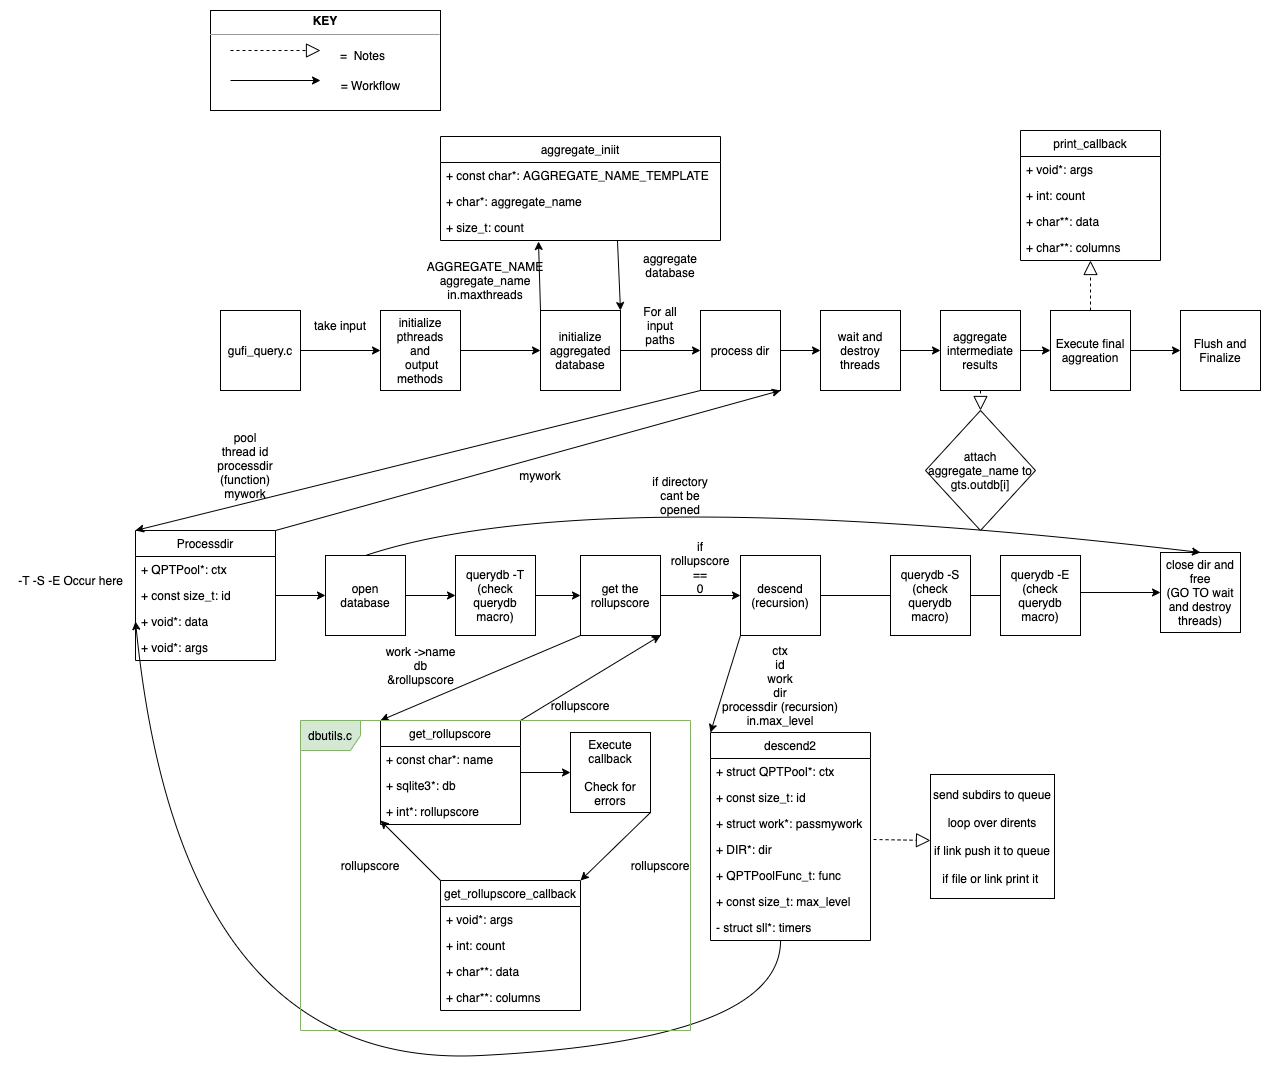
\includegraphics[width=1.0\textwidth]{images/gufi_query.png}
\caption{\label{fig:gufi_query}Workflow of gufi\_query}
\end{figure}

